%% Packages initialisation
\documentclass[10pt,compress]{beamer}
\usepackage[utf8]{inputenc}               % Enable UTF-8 compatible typing
\usepackage{hyperref}                     % Interactive PDF
\usepackage{listings}
\usepackage{xcolor}
\usepackage{multirow}
\usepackage{amssymb,mathtools}       % For mathematical writing
\usepackage{tikz}                    % Drawing trees
\usetikzlibrary{trees,shapes.multipart}
\usepackage[round]{natbib}


%% Use the default theme
\usetheme{default}

%% Colours block environment headings
\useinnertheme{rectangles}
\mode<beamer>{\setbeamertemplate{blocks}[rounded][shadow=false]} 
\setbeamercolor{block title}{bg=blue!10,fg=black}
\makeatletter
\pgfdeclareverticalshading[lower.bg,upper.bg]{bmb@transition}{200cm}{%
  color(0pt)=(upper.bg); color(2pt)=(upper.bg); color(4pt)=(upper.bg)}
\makeatother

%% Enable slide numbering
\makeatletter
\setbeamertemplate{footline}
{
  \leavevmode%
  \hbox{%
  \begin{beamercolorbox}[wd=.3\paperwidth,ht=2.25ex,dp=1ex,left]{author in head/foot}%
    \hspace*{2ex}\usebeamerfont{author in head/foot}\insertshortauthor~~\beamer@ifempty{\insertshortinstitute}{}{(\insertshortinstitute)}
  \end{beamercolorbox}%
  \begin{beamercolorbox}[wd=.5\paperwidth,ht=2.25ex,dp=1ex,center]{title in head/foot}%
    \usebeamerfont{title in head/foot}\insertshorttitle
  \end{beamercolorbox}%
  \begin{beamercolorbox}[wd=.1\paperwidth,ht=2.25ex,dp=1ex,center]{date in head/foot}%
    \usebeamerfont{date in head/foot}\insertshortdate{}
  \end{beamercolorbox}
  \begin{beamercolorbox}[wd=.1\paperwidth,ht=2.25ex,dp=1ex,right]{date in head/foot}%
    \usebeamerfont{date in head/foot}\insertframenumber /\inserttotalframenumber\hspace*{2ex}
  \end{beamercolorbox}}%
  \vskip0pt%
}
\makeatother

%% Hide navigation buttons
\beamertemplatenavigationsymbolsempty

%% Lstlisting style
\lstset{
 backgroundcolor=\color{white},   % choose the background color; you must add \usepackage{color} or \usepackage{xcolor}
 basicstyle=\ttfamily\footnotesize,        % the size of the fonts that are used for the code
 keywordstyle=\bfseries,
 commentstyle=\itshape,
 % SL: lstinline doesn't work properly if breakatwhitespace is not set to true
 breakatwhitespace=true,         % sets if automatic breaks should only happen at whitespace
 breaklines=true,                 % sets automatic line breaking
 captionpos=b,                    % sets the caption-position to bottom
 escapeinside={\#*}{*\#},          % if you want to add LaTeX within your code
 extendedchars=true,              % lets you use non-ASCII characters; for 8-bits encodings only, does not work with UTF-8
 frame=none,	                   % adds a frame around the code
 keepspaces=true,                 % keeps spaces in text, useful for keeping indentation of code (possibly needs columns=flexible)
 numbers=none,                    % where to put the line-numbers; possible values are (none, left, right)
 rulecolor=\color{black},         % if not set, the frame-color may be changed on line-breaks within not-black text (e.g. comments (green here))
 showspaces=false,                % show spaces everywhere adding particular underscores; it overrides 'showstringspaces'
 showstringspaces=false,          % underline spaces within strings only
 showtabs=false,                  % show tabs within strings adding particular underscores
 tabsize=1,	                   % sets default tabsize to 2 spaces
 title=\lstname,                   % show the filename of files included with \lstinputlisting; also try caption instead of title
 caption={},
 belowcaptionskip=-1\baselineskip,
 xleftmargin=0.1\parindent,
 columns=fullflexible
}

\lstdefinelanguage{Links}{% 
  morekeywords={typename, fun, op, var, if, this, true, false, else, case, switch, handle, handler, shallowhandler, open, do, sig},%
  sensitive=t, % 
  keywordstyle=\color{red},
  emph={Fail,Choose,Return},
  emphstyle={\color{blue}},
  comment=[l]{\#},% 
  escapeinside={(*}{*)},%
  morestring=[d]{"}%
 }

\newcommand{\textapprox}{{\fontfamily{ptm}\selectfont\texttildelow}}
\newcommand{\wildarrow}{\linksify{\textapprox{}>}}
% Links style
\lstdefinestyle{links}{
  basicstyle=\linespread{1.0}\ttfamily\footnotesize,
  language=Links,
  literate= {~>}{{\wildarrow}}1
}

\lstset{style={links}}

%% Checkmark
\def\checkmark{\tikz\fill[scale=0.4](0,.35) -- (.25,0) -- (1,.7) -- (.25,.15) -- cycle;}

%% Meta information
\author[Daniel Hillerström]{Daniel Hillerström\\\footnotesize{\href{mailto:daniel.hillerstrom@ed.ac.uk}{daniel.hillerstrom@ed.ac.uk}}\\\href{http://homepages.inf.ed.ac.uk/s1467124}{http://homepages.inf.ed.ac.uk/s1467124}}
\title{Towards Compilation of Affine Algebraic Effects Handlers}
%\subtitle{\textit{\dots with slide numbering!}}
\institute{The University of Edinburgh}
\date{\today}

%% Slides
\begin{document}
% Front slide
\begin{frame}[plain]
  \maketitle
\end{frame}

\begin{frame}
  \frametitle{The Links language}
The code examples in this talk are written in Links\footnote{ref. \citet{Cooper2006}}:
\begin{itemize}
  \item Pure, functional, web-oriented, research programming language.
  \item Sort of JavaScript syntax with sane semantics.
  \item Developed at the University of Edinburgh
  \item Conceived to solve the \emph{impedance mismatch problem} in web-programming.
  \item Best thing about Links: \uncover<2->{\textbf{It has no users}}
\end{itemize}
\end{frame}

\begin{frame}
  \frametitle{Programs are effectful}
Virtually, every program comprise an \alert<1->{effectful} component, e.g.
\begin{itemize}
  \item raise exceptions
  \item perform input/output
  \item mutate some state
  \item fork threads
  \item non-determinism
  \item \dots and so forth 
\end{itemize}
In most programming languages effects are dealt with \emph{implicitly}.

Algebraic effects and handlers provide a modular abstraction for modelling and controlling effects \emph{explicitly}.
\end{frame}

\begin{frame}[fragile]
  \frametitle{Algebraic effects by example: A coin toss\footnote{The example is adopted from \citet{Kammar2013}}}
  \begin{block}{Algebraic effects}
    An algebraic effect is a collection of abstract operations.    
  \end{block}
For example, nondeterminism is given by a single operation $nondet = \{{\color{blue}{Choose}} : \text{Bool}\}$
\vspace{1cm}
\begin{columns}
\begin{column}{0.5\textwidth}
An effectful coin toss:
\begin{lstlisting}
fun toss() {
  if (do Choose) Heads
  else Tails
} 
\end{lstlisting}
\end{column}
\begin{column}{0.5\textwidth}
Visualised as a computation tree:
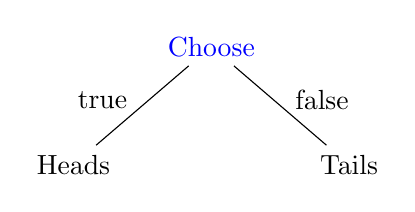
\begin{tikzpicture}[level distance=1.5cm,
level 1/.style={sibling distance=3.5cm},
level 2/.style={sibling distance=1cm}]
%\tikzstyle{every node}=[circle,draw]

\node (Root) [blue,rectangle] {Choose}
      child { node[draw=none] { Heads } 
        edge from parent node [draw=none,left,xshift=-2.0,yshift=2.0] { true }
      }
      child { node[draw=none] { Tails } 
        edge from parent node [draw=none,right,xshift=2.0,yshift=2.0] { false }
      };
\end{tikzpicture}
\end{column}
\end{columns}
\end{frame}

\begin{frame}[fragile]
  \frametitle{Effect handlers by example: A coin toss}
\begin{block}{Handlers}
A handler instantiates abstract operations with a concrete implementation.
\end{block}
\begin{columns}
\begin{column}{0.5\textwidth}
\begin{lstlisting}
fun toss() {
  if (do Choose) Heads
  else Tails
}

handler alwaysHeads {
  case Choose(k) -> k(true)
  case Return(x) -> x
}
\end{lstlisting}
\end{column}
\begin{column}{0.5\textwidth}
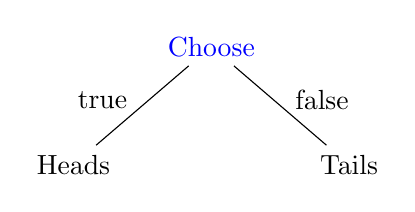
\begin{tikzpicture}[level distance=1.5cm,
level 1/.style={sibling distance=3.5cm},
level 2/.style={sibling distance=1cm}]
%\tikzstyle{every node}=[circle,draw]

\node (Root) [blue,rectangle] {Choose}
      child { node[draw=none] { Heads } 
        edge from parent node [draw=none,left,xshift=-2.0,yshift=2.0] { true }
      }
      child { node[draw=none] { Tails } 
        edge from parent node [draw=none,right,xshift=2.0,yshift=2.0] { false }
      };
\end{tikzpicture}\\
$\Longrightarrow$ Heads
\end{column}
\end{columns}
Here \lstinline$k$ is the continuation of \lstinline$do Choose$.
\end{frame}

\begin{frame}
  \frametitle{Project overview}
I'm interested in making effect handlers a practical programming model.
\begin{description}
  \item[Phase 1] Front-end: handlers and row types\footnote{c.f. \citet{Hillerstrom2016}} $\checkmark$
  \item[Phase 2] Back-end: compile handlers to efficient, native code.
  \item[Phase 3] Rebuild Links' concurrency model in terms of handlers
\end{description}
Continuations are the main performance bottleneck.
OCaml multicore\footnote{ref. \citet{Dolan2015}} provides an efficient implementation of \emph{linear} handlers.
My plan is to translate Links IR to OCaml Lambda IR.
\end{frame}

% \begin{frame}
%   \frametitle{Some implementations\footnote{First-class}}
% \begin{itemize}
%   \item Bauer and Pretnar's \emph{Eff} 
%   \item Lindley, McBride and McLaughlin's Frank
%   \item McBride's shonky
%   \item OCaml's effects/multicore implementation
%   \item Hillerström and Lindley's Links
% \end{itemize}
% OCaml provides an efficient implementation of \emph{linear} handlers.
% \end{frame}

\begin{frame}[fragile]
  \frametitle{Categorising handlers}
  \begin{table}
    \begin{tabular}{l l}
   \alt<2->{\textbf{Exception}}{Exception}\footnote{where $exception = \{{\color{blue}{Fail}} : Void\}$} &
\begin{lstlisting}
handler maybeResult {
  case Fail(k)   -> Nothing
  case Return(x) -> Just(x)
}
\end{lstlisting}
\\
      \hline
      \alt<2->{\textbf{Linear}}{Linear}    & 
\begin{lstlisting}
handler randomResult {
  case Choose(k) -> k(random() > 0.5)
  case Return(x) -> x
}
\end{lstlisting} \\
      \hline
      Multi-shot & 
\begin{lstlisting}
handler allResults {
  case Choose(k) -> k(true) ++ k(false)
  case Return(x) -> [x]
}
\end{lstlisting}
   \end{tabular}
  \end{table}
\uncover<2->{\textbf{Affine} handlers invoke their continuations at most once.}

\uncover<2->{Idea: Use the type system to track the nature of handlers, and specialise the run-time implementations during code generation.}
\end{frame}

\begin{frame}[fragile]
  \frametitle{Composing handlers by example: Drunk coin toss}
Consider a drunkard tossing a coin\footnote{Technical detail: \lstinline$switch(do Fail) \{ \}$ required for example to type check.}:
\begin{lstlisting}
fun drunkToss() {
  if (do Choose) toss()
  else do Fail
}
\end{lstlisting}
We may compose handlers to fully interpret \lstinline$drunkToss$: \lstinline$randomResult(maybeResult(drunkToss))$.
\vspace{0.5cm}

Possible outcomes: $\{$\lstinline$Just(Heads)$$,$\lstinline$Just(Tails)$$,$\lstinline$Nothing$$\}$.
\end{frame}

\begin{frame}[fragile]
  \frametitle{Runtime stack of handlers}
  Composition gives rise to stack of handlers at runtime:
\vfill
\begin{columns}
\begin{column}{0.5\textwidth}
\lstinline$randomResult(maybeResult(drunkToss))$
\end{column}
\begin{column}{0.5\textwidth}
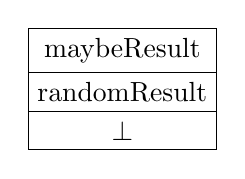
\begin{tikzpicture}[stack/.style={rectangle split, rectangle split parts=#1,draw, anchor=center}]
\node[stack=3]  {
\nodepart{one}maybeResult
\nodepart{two}randomResult
\nodepart{three}$\bot$
};
\end{tikzpicture}
\end{column}
\end{columns}
\vfill
Handling \lstinline$Choose$ in \lstinline$drunkToss$ causes the stack to be unwinded.
\end{frame}

\begin{frame}
  \frametitle{Optimisations}
  The stack representation is simple, but inefficient for large compositions.
  OCaml does not perform optimisations for handlers.
\vfill
  Solution: Rediscover classical optimisations in the context of handlers:
  \begin{itemize}
    \item Fusion
    \item Inlining
    \item Reordering of handlers
  \end{itemize}
\end{frame}

\begin{frame}[fragile]
  \frametitle{Optimisation: Fusion}
  \begin{block}{Criterion for handler fusion}
    If two adjacent handlers handle a disjoint set of operations, then they can be fused.
  \end{block}
\vfill
\begin{columns}
\begin{column}{0.6\textwidth}
% Before fusion
\begin{onlyenv}<1-1>
\begin{lstlisting}
handler maybeResult {
  case Fail(k)   -> Nothing
  case Return(x) -> Just(x)
}
\end{lstlisting}

\begin{lstlisting}
handler randomResult {
  case Choose(k) -> k(random() > 0.5)
  case Return(x) -> x
}
\end{lstlisting}
\end{onlyenv}
% After fusion
\begin{onlyenv}<2->
\begin{lstlisting}
handler maybeRandomResult {
  case Fail(k)   -> Nothing
  case Choose(k) -> k(random() > 0.5)
  case Return(x) -> var y = Just(x); y
}
\end{lstlisting}
\end{onlyenv}
\end{column}
\begin{column}{0.4\textwidth}
% Before fusion
\begin{onlyenv}<1-1>
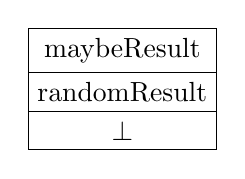
\begin{tikzpicture}[stack/.style={rectangle split, rectangle split parts=#1,draw, anchor=center}]
\node[stack=3]  {
\nodepart{one}maybeResult
\nodepart{two}randomResult
\nodepart{three}$\bot$
};
\end{tikzpicture}
\end{onlyenv}
% After fusion
\begin{onlyenv}<2->
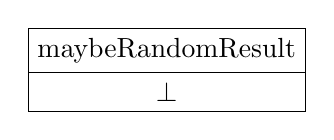
\begin{tikzpicture}[stack/.style={rectangle split, rectangle split parts=#1,draw, anchor=center}]
\node[stack=2]  {
\nodepart{one}maybeRandomResult
\nodepart{two}$\bot$
};
\end{tikzpicture}
\end{onlyenv}
\end{column}
\end{columns}
\end{frame}

\begin{frame}[fragile]
  \frametitle{Optimisation: Inlining}
  \begin{block}{Criterion for handler inlining}
    A linear handlers can be inlined if
    \begin{itemize}
      \item It invokes continuations in tail-position\footnote{There are ways to sometimes relax this requirement}
      \item The handler is the top-element ($\top$)
    \end{itemize}
  \end{block}
\vfill
\begin{columns}
\begin{column}{0.52\textwidth}
\begin{lstlisting}
handler maybeResult {
  case Fail(k)   -> Nothing
  case Return(x) -> Just(x)
}
\end{lstlisting}

\begin{onlyenv}<1-5>
\begin{lstlisting}
handler randomResult {
  case Choose(k) -> k(random() > 0.5)
  case Return(x) -> x
}
\end{lstlisting}
\end{onlyenv}
\end{column}
\begin{column}{0.48\textwidth}
% Before reordering
\begin{onlyenv}<1-4>
\begin{lstlisting}
(*\alert<3-3>{randomResult}*)(
(*  \alert<2-2>{maybeResult}*)(
    fun() {
     if (do Choose) toss()
     else do Fail
    }))
\end{lstlisting}
\end{onlyenv}
% After reordering
\begin{onlyenv}<5-5>
\begin{lstlisting}
maybeResult(
  randomResult(
    fun() {
     if (do Choose) toss()
     else do Fail
    }))
\end{lstlisting}
\end{onlyenv}
% After inlining
\begin{onlyenv}<6-6>
\begin{lstlisting}
maybeResult(
 fun() {
  if (random() > 0.5) 
   toss()[random()>0.5/do Choose]
  else do Fail
 }))
\end{lstlisting}
\end{onlyenv}
\end{column}
\end{columns}
\only<2-2>{\alert<2-2>{Cannot inline \lstinline$maybeResult$: it is not linear}}

\only<3-4>{\alert<3-4>{Cannot inline linear \lstinline$randomResult$: it is not $\top$}}

\uncover<3-4>{If we reorder the two handlers, then we can inline \lstinline$randomResult$}
\end{frame}

\begin{frame}
  \frametitle{Summary}
  \begin{itemize}
    \item Handlers provide a great abstraction for generic programming.
    \item I get native baseline performance for free from OCaml.
    \item We need to rethink classical optimisations in the context of handlers
    \item I have some ideas, that look good on paper, for optimisations.
  \end{itemize}
\end{frame}

% Bibliography
\begin{frame}
  \frametitle{References}
  \nocite{*}
  \bibliographystyle{abbrvnat}
  \bibliography{references}
\end{frame}
\end{document}